\section{Execution-based evaluation}
\label{sec:protocol}

\paragraph{Executed program.} Every system delivers a CadQuery program \citep{cadquery}. We run it in a fresh sandboxed process with no network access and a 900\,s limit, take its result solid, and check OCC validity of the shape and of every solid it contains. A program that fails to build, builds an invalid solid, exceeds the limit, or is missing is a failed delivery.

\paragraph{Judge.} The executed solid is tessellated and compared with the target, normalized so that its largest extent spans $[-1,1]$. When both meshes are closed and consistently oriented, IoU is computed exactly with manifold booleans \citep{manifold3d}; otherwise it is a seeded Monte-Carlo estimate in which inside-ness of the reconstruction is the generalized winding number \citep{jacobson2013winding}, so a tessellation cracked by float round-off is not judged as a hollow shell. \textbf{Validity-gated IoU} is the IoU of the executed solid if the delivery succeeded and 0 otherwise. Every cohort part stays in every denominator.

\paragraph{Cohorts.} All parts are hard-tier CADBench \citep{doris2026cadbench} solids from two splits, benchA and benchE, drawn by seeded shuffles that exclude every source model already used in any earlier set. Development used separate sets (\cref{app:cohorts}). \textbf{fresh2} (150 + 150 parts) was drawn after development for the optimizer study; \textbf{40 reserved parts} (20 + 20) were drawn from fresh2's manifest before any fresh2 outcome existed and used for the agent study; \textbf{fresh3} (20 + 20) was drawn after the revised tools and their protocol were frozen. The optimizer's outcomes on fresh2's other 260 parts were seen before the agent studies began; fresh3 is the only cohort unseen by every analysis.

\paragraph{Statistics.} All comparisons are paired over parts. Repeated runs or episodes are averaged within part first. Intervals are nominal 95\% bootstrap intervals that resample parts within split \citep{efron1993bootstrap}. Tests are exact two-sided sign tests on per-part differences; a part counts as better or worse when its difference exceeds $\pm0.005$ in the optimizer study and $\pm10^{-9}$ in the agent studies, and as neutral otherwise. Holm correction is applied within each declared family (stated per study).

\paragraph{Preregistration and amendments.} Each study's arms, cohort, primary and secondary comparisons and analysis code were committed before its runs. Changes made after outcomes existed are recorded as dated amendments, reported in the main text with their effect, and listed with every exclusion and rerun in \cref{app:log}.

\begin{figure}[t]
\centering
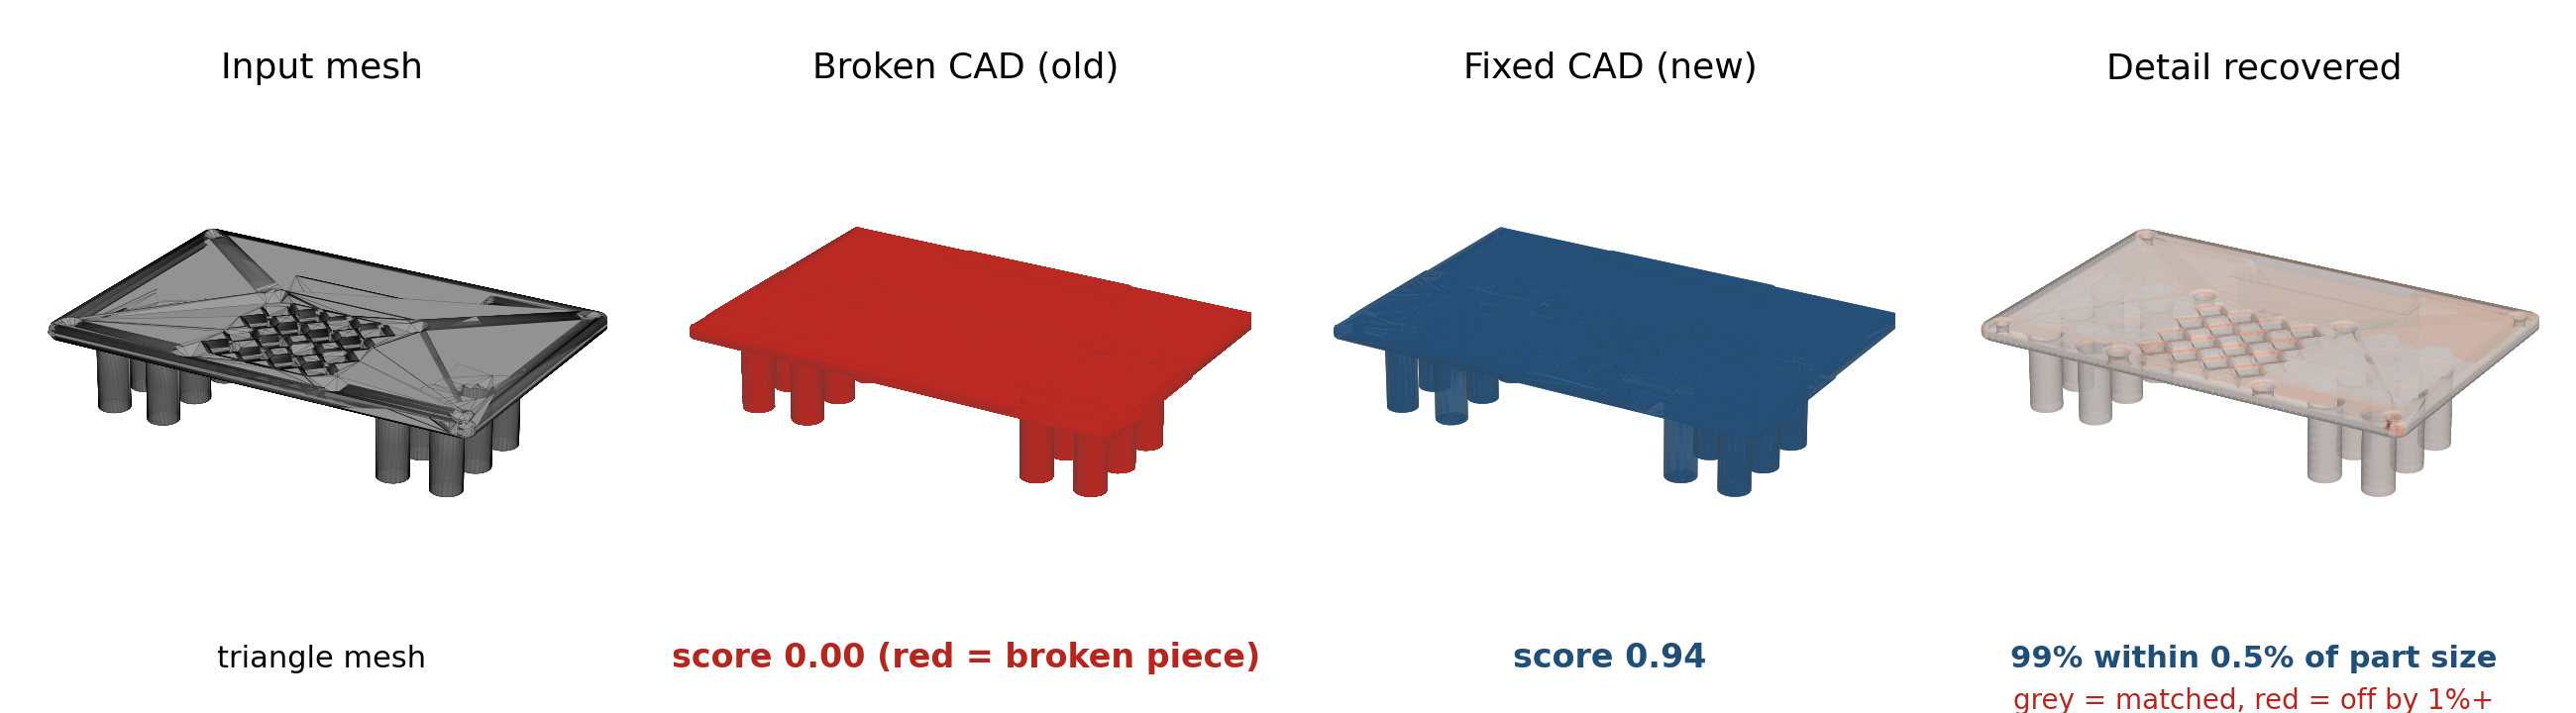
\includegraphics[width=\linewidth]{figures/detail.png}
\caption{A development part (not from any evaluation cohort). Left to right: the input mesh; the program written by the optimizer's search, which stacks 208 overlapping solids of which 34 are OCC-invalid (red) and therefore scores 0; the program delivered by the execution check, a fused rewrite with one valid solid (IoU 0.94, as recorded by the pipeline); the input surface colored by distance to that delivery (grey within 0.5\% of the part size).}
\label{fig:detail}
\end{figure}
